\section{V5}
\subsection{Konfidenzintervall}
$P(E(x)) \in \displaystyle [\bar{x_n} - 1.96 \frac{\hat{\sigma}}{\sqrt{N}}, \bar{x_n} + 1.96 \frac{\hat{\sigma}}{\sqrt{N}}]$ = 0.95

\textbf{Interpretation des 95\% Konfidenzintervalls}
\begin{itemize}
	\item Interpretation (\underline{frequentistisch}): In 95\% aller Stichproben vom Umfang N liegt der wahre Erwartungswert in dem oben angegebenen Intervall.
	\item Alternativ (frequentistisch): 95\% der so konstruierten Konfidenzintervalle enthalten den wahren Wert
	\item Interpretation (\underline{Bayesianisch}): Mit 95\% Sicherheit (nicht Wahrscheinlichkeit!) liegt der wahre Erwartungswert in diesem Intervall.
	\item Für eine spezielle gegebene Stichprobe können wir jedoch nicht sagen, ob der wahre Wert in diesem Intervall liegt oder nicht. In der Regel gibt es auch keine Möglichkeit, dies anderweitig zu zeigen.
\end{itemize}

\subsection{Logik des statistischen Testens, Testdurchführung und Interpretation}
\textbf{Beobachtung:} Unterschied zwischen zwei Gruppen (z.B. zwei Therapievarianten, zwei genetischen Varianten A und B (bei Variante A mehr Ereignisse))
\\\\
\textbf{Skeptiker:} Dieses Ergebnis ist zufällig!
\\\\
\textbf{Annahme:} Der Skeptiker hat recht. Es gibt keinen Unterschied (Nullhypothese).
\\\\
\textbf{Frage:} Wie gut können Zufallseffekte die Daten erklären? Wie wahrscheinlich ist meine Beobachtung, wenn die Nullhypothese war ist (p-Wert)?
\\\\
\textbf{Maßzahl:} Wahrscheinlichkeit p (p-Wert) den beobachteten Unterschied (oder noch extremere Abweichungen von der Nullhypothese) rein zufällig zu erhalten.

\textbf{Statistische Schlussweise:} Wenn p klein ist...
\begin{itemize}
	\item Etwas sehr Unwahrscheinliches ist geschehen
	\item Unsere Annahme (Nullhypothese) ist falsch
\end{itemize}

Je kleiner p, desto unplausibler ist die Nullhypothese\\
\textbf{Konvention:} p $< \alpha$ = 0.05 („signifikant“) $\rightarrow$ Nullhypothese ablehnen

\newpage
\textbf{Allgemeine Konstruktion eines statistischen Tests:}
\begin{enumerate}
	\item Auswahl eines Effektmaßes (z.B. (standardisierte) Mittel-
wertsdifferenz)
	\item Bestimme zugehörige Verteilung unter der Nullhypothese
	\item Lege extreme Abweichungen von der Nullhypothese fest (z.B. zweiseitig oder einseitig)
	\item Berechne die beobachtete Teststatistik z
	\item Berechne den p-Wert aus z und der Verteilung unter der Nullhypothese
\end{enumerate}

\subsection{Typ I und Typ II Fehler, Einfluß der Fallzahl}
\textbf{Konfidenzniveau}
\begin{itemize}
	\item Bemerkung 1: $\alpha$ wird Typ 1 Fehler genannt.
	\item Bemerkung 2: Statistische Tests korrespondieren fast immer zu Berechnungen von 95\% Konfidenzintervallen. Die Nullhypothese kann verworfen werden, wenn deren Effekt außerhalb des Konfidenzintervalls des beobachteten Effekts liegt.
	\item Bemerkung 3: Wenn p groß ist, kann man gar nichts schlussfolgern. Die Annahme, dass dann die Nullhypothese gilt bzw. gar bewiesen wurde, ist ein (leider sehr weit verbreiteter) Irrtum.
	\item Bemerkung 4: Statistische Signifikanz hat nichts mit Relevanz zu tun. Selbst die kleinsten Effekte können bei großen Fallzahlen signifikant werden.
\end{itemize}

\textbf{Power}
\begin{itemize}
	\item Neben dem Typ-1 Fehler $\alpha$ gibt es auch einen Typ-2 Fehler $\beta$. Er beschreibt die Wahrscheinlichkeit, eine falsche Nullhypothese nicht aufdecken zu können.
	\item 1-$\beta$ heißt Power und sollte möglichst groß sein (Studienplanung, für klinische Studien $\sim$80\%)
	\item Die Power hängt ab von der Wahl des Signifikanzniveaus $\alpha$, von der Stärke der Abweichung von der Nullhypothese (Effektstärke) und der Fallzahl.
	\item Kleine Signifikanzniveaus und Effektstärken erfordern eine große Fallzahl um eine akzeptable Power zu erreichen (vergleiche später)
\end{itemize}

\subsection{Problem des multiplen Testens und Korrekturmöglichkeiten}
\begin{itemize}
	\item Bei einem Test beträgt die Wahrscheinlichkeit, dass man die Nullhypothese fälschlicherweise ablehnt $\alpha$
	\item typischer Wert für $\alpha$ ist 0,05
	\item beim mehrmaligen Testen von Hypothesen innerhalb einer Stichprobe kommt es zu einer sogenannten $\alpha$-Fehler-Kumulierung
	\item Testet man zum Beispiel 1 Mio. genetische Varianten erhält man schon durch Zufall 50.000 signifikante Ergebnisse
\end{itemize}

\textbf{Korrekturmöglichkeiten}
\begin{itemize}
	\item Kontrolle der family-wise error rate (FWER): Bonferroni, Bonferroni-Holm
	\item False discovery rate (FDR): Benjamini-Hochberg, Schätzen des Anteils wahrer Nullhypothesen
\end{itemize}

\subsection{Faktoren für die Auswahl des richtigen Tests}
Statistische Tests müssen passend zum Variablentyp gewählt werden.

\underline{Gepaarte versus ungepaarte Vergleiche}
\begin{itemize}
	\item Ungepaart: Vergleich zwischen verschiedenen Gruppen
	\item Beispiele:
	\begin{itemize}
		\item Geschlechter
		\item Fälle versus Kontrollen
		\item verschieden behandelte Individuen
	\end{itemize}
	\item Gepaart: Vergleiche innerhalb eines Individuums oder Entität
	\item Beispiele:
	\begin{itemize}
		\item rechtes gegen linkes Auge/Hand
		\item wiederholte Messungen innerhalb von Probanden
		\item gematchte Fälle und Kontrollen
	\end{itemize}
\end{itemize}

\textbf{Überblick (Vergleich stetiger Variablen)}\\
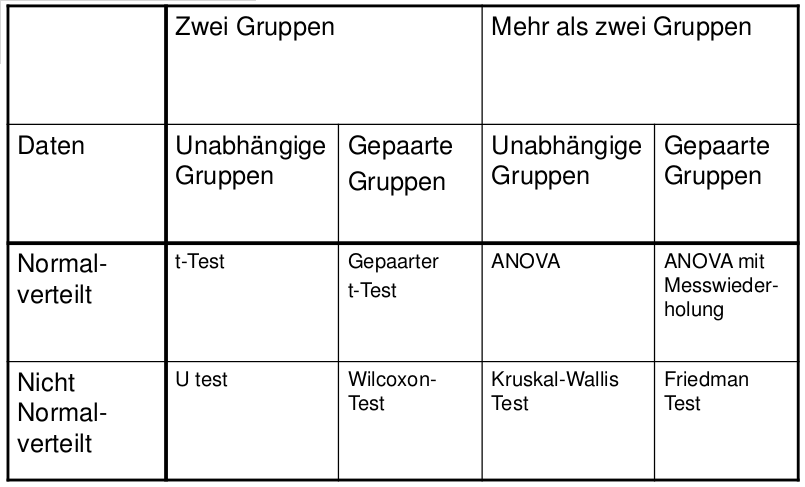
\includegraphics[width=1.00\textwidth]{lectures/V5/pix/stet_var.png}
\\
\textbf{Überblick (Vergleich binärer Variablen)}\\
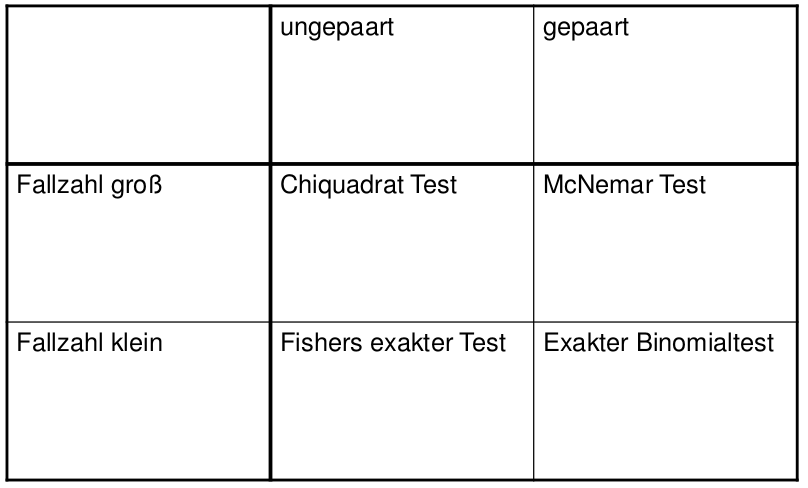
\includegraphics[width=1.00\textwidth]{lectures/V5/pix/bin_var.png}

\subsection{Zusammenhangsmaße auf Vierfeldertafeln}
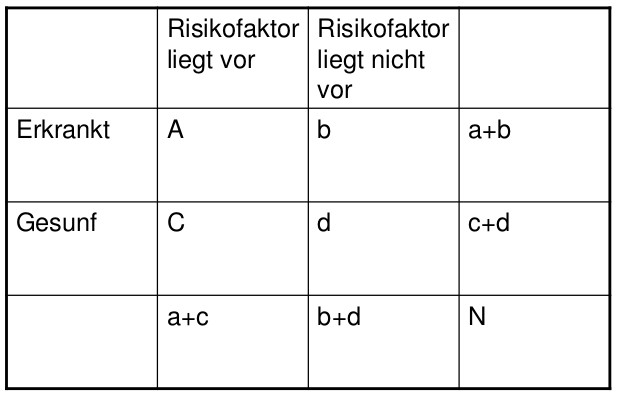
\includegraphics[width=1.00\textwidth]{lectures/V5/pix/vft.png}
\textbf{Maße:}
\begin{itemize}
	\item Absolute Risikodifferenz: $\displaystyle ARD=\frac{a}{a+c}-\frac{b}{b+d}$
	\item Relatives Risiko: $RR=\displaystyle \frac{\displaystyle \frac{a}{a+c}}{\displaystyle \frac{b}{b+d}}$
	\item Odds-ratio: $\displaystyle OR=\frac{ad}{bc}$
\end{itemize}

\textbf{Warum sollte man die Odds-ratio verwenden?}
\begin{itemize}
	\item ARD und RR hängen vom Basisrisiko ab $\rightarrow$ Vergleich zwischen Gruppen kann irreführend sein (wie in unserem Emesis-Beispiel)
	\item OR ist unabhängig vom Basisrisiko $\rightarrow$ kann zwischen Gruppen verglichen werden
	\item Die Nullhypothese des Chiquadrat-Tests ist OR=1 $\rightarrow$ OR ist das zum Chiquadrat-Test passende Effektmaß
\end{itemize}

\newpage
\subsection{Korrelation, Scheinkorrelation und Confounder}
\textbf{Pearsons Korrelationskoeffizient}
$r(X,Y)=\displaystyle \frac{var(X+Y) - var(X) - var(Y)}{2 \sqrt{var(X)} \sqrt{var(Y)}}$
\\\\
\textbf{Eigenschaften:}
\begin{enumerate}
	\item Misst den Grad der linearen Abhängigkeit zwischen X und Y
	\item $-1 \leq r(X,Y) \leq 1$
	\item r(X,Y) ist invariant unter linearer Transformation von X und Y
	\item Falls Y=aX+b dann r(X,Y)=sign(a)
	\item Misst nicht die Übereinstimmung (Konkordanz) von X und Y
\end{enumerate}

\textbf{Grobe Einteilung der Stärke des linearen Zusammenhangs:}
\begin{itemize}
	\item $|r|$ $<$ 0,3 schwach
	\item 0,3 $\leq$ $|r|$ $<$ 0,6 mittel
	\item 0,6 $\leq$ $|r|$ $<$ 0,8 stark
	\item 0,8 $\leq$ $|r|$ $<$ 1,0 sehr stark
	\item $|r|$ = 1,0 perfekter Zusammenhang
\end{itemize}

Kombination nicht vergleichbarer Stichproben führt zu \textbf{Scheinkorrelation}. Größen die Scheinkorrelationen erzeugen heißen \textbf{Confounder}.

\subsection{Aufgaben zur Übung 5}